\graphicspath{{./ch_C13_dephasing_LDE/figures/}}


\chapter{Analysis of a quantum memory with optical interface in diamond }
\label{ch:CDL}

\begin{center} 
    \vspace{-1cm} {M.S.~Blok, N.~Kalb, A.~Reiserer, T.H.~Taminiau and R.~Hanson} 
\end{center}


{\renewcommand{\thefootnote}{}\footnote{This chapter has been accepted in
    {\em Faraday Discussions} (2015).}}


\vspace{-0.5cm} 
abstract ~\cite{Gao_NatPhoton_2015,Kimble_Nature_2008,Moehring_Nature_2007,Ritter_Nature_2012,Hofmann_Science_2012,Bernien_Nature_2013,Bennett_Phys.Rev.Lett._1996,Campbell_Phys.Rev.Lett._2008,Briegel_Phys.Rev.Lett._1998,Childress_Phys.Rev.Lett._2006,Childress__2013,Togan_Nature_2010,Bernien_Nature_2013,Pfaff_Science_2014,Jelezko_Phys.Rev.Lett._2004,Dutt_Science_2007,Neumann_Science_2008a,Smeltzer_Phys.Rev.A_2009,Fuchs_NatPhys_2011,vanderSar_Nature_2012,Taminiau_Phys.Rev.Lett._2012,Maurer_Science_2012,Tamarat_NewJ.Phys._2008,Robledo_Nature_2011,Togan_Nature_2010,Kolkowitz_Phys.Rev.Lett._2012,Zhao_NatNano_2012,Taminiau_NatNano_2014,Barrett_Phys.Rev.A_2005}
Single defect centers in diamond have emerged as a powerful platform for quantum optics experiments and quantum information processing tasks1. Connecting spatially separated nodes via optical photons2 into a quantum network will enable distributed quantum computing and long-range quantum communication. Initial experiments on trapped atoms and ions as well as defects in diamond have demonstrated entanglement between two nodes over several meters3-6. To realize multi-node networks, additional quantum bit systems that store quantum states while new entanglement links are established are highly desirable. Such memories allow for entanglement distillation, purification and quantum repeater protocols that extend the size, speed and distance of the network7-10. However, to be effective the memory must be robust against the entanglement generation protocol, which typically must be repeated many times. Here we evaluate the prospects of using carbon nuclear spins in diamond as quantum memories that are compatible with quantum networks based on single nitrogen vacancy (NV) defects in diamond. We present a theoretical framework to describe the dephasing of the nuclear spins under repeated generation of NV spin-photon entanglement and show that quantum states can be stored during hundreds of repetitions using typical experimental coupling parameters. This result demonstrates that nuclear spins with weak hyperfine couplings are promising quantum memories for quantum networks.
\clearpage

\section{Introduction}

Spins associated with the nitrogen-vacancy (NV) center, an atomic defect in diamond, have recently emerged as a promising platform for quantum networks1,11. The NV-center’s long-lived electron spin state (S=1) can be controlled by magnetic resonance and can be initialized and read out optically. At cryogenic temperatures (< 10 K), coherent optical transitions allow for the generation of spin-photon entanglement12 and of entanglement between spatially separated NV center electron spins6,13. 

In addition, the electron spin couples to nuclear spins in the environment through the hyperfine interaction. Control over the host nitrogen spin and over multiple nearby 13C spins has been demonstrated14-20. As these nuclear spins can be well isolated from their environments, coherence times of more than one second have been demonstrated21, making them interesting candidates for quantum network memories. 

A major challenge for realizing quantum memories based on nuclear spins is to overcome the dephasing that is introduced while using the electron spin as an optical interface to generate spin-photon entanglement. Consider the general case of an entanglement protocol that is inherently probabilistic due to lossy optical channels. The protocol therefore must be repeated many times in order to establish an entanglement link between adjacent network nodes. Whenever the entanglement attempt fails, the electron spin is projected in a random state. A fast and practical solution is to re-initialize the spin by optical pumping after each repetition. Because the exact time at which the electron spin is reset is uncertain (optical pumping is a stochastic process) and the electron-nuclear interaction is always present, the electron reset can cause nuclear spin dephasing (Fig 1). A promising route to overcome this dephasing of the quantum memory is to use relatively distant $^{13}C$ spins with weak hyperfine couplings, which are less sensitive to fluctuations of the electron spin.  

In this manuscript we explore the storage of quantum states in 13C spins during the repeated generation of NV spin-photon entanglement. We first demonstrate a method to directly measure the frequency difference df for the electron-state-dependent nuclear spin precessions, which governs the nuclear dephasing (Fig 1)22. We then analyze the spin-photon entanglement protocol, develop a model to describe the dephasing of nuclear spins, and calculate the fidelity of nuclear spin quantum memories with realistic coupling parameters under many repetitions of the entanglement protocol. 


\section{Control and Characterization of nuclear spins in diamond}
\begin{figure*}
	\centering
	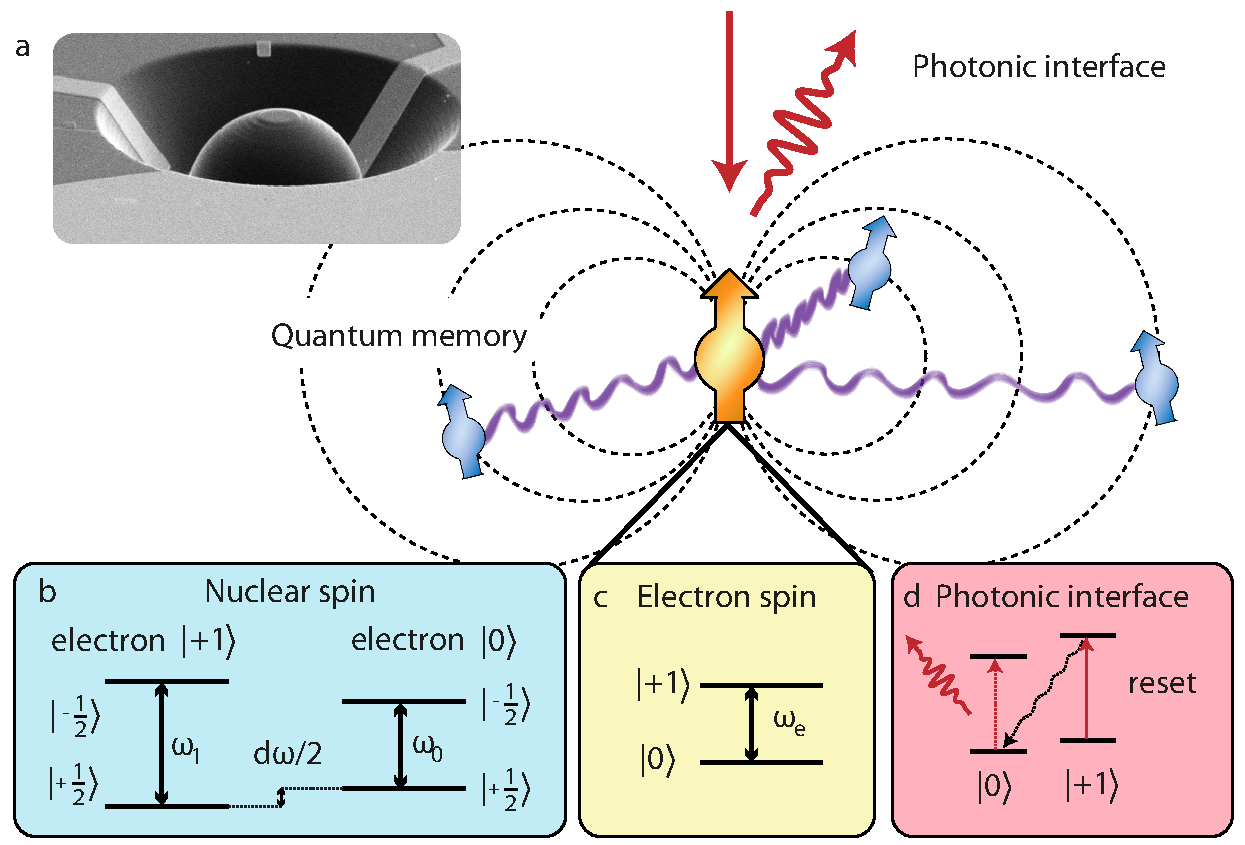
\includegraphics{Fig1}
	\caption{\label{fig:cdl-fig1} \textbf{} (a) }
\end{figure*}

We start by discussing the experimental methods to control the NV center and nearby $^{13}C$  nuclear spins. We then introduce a Ramsey-spectroscopy method to directly determine the frequency df and characterize four candidate $^{13}C$  spins near a single NV-center. These experimental results highlight the universal presence of controllable nuclear spin memories and provide a realistic set of input parameters for the theoretical calculations.

At the heart of the experiment is a single Nitrogen-Vacancy (NV) center in high purity (Type IIa) single-crystal diamond grown by chemical-vapor-deposition. The diamond is held at a temperature of \textit{T} = 4.2 K in a Helium bath cryostat. The diamond has a natural abundance (1.1\%) of 13C spins (\textit{I} = 1/2) in an otherwise $^{12}C$ spin-free lattice. The NV electronic spin is polarized and measured optically by spin-selective resonant excitation12,23,24. To obtain high single-shot readout fidelities, a solid-immersion lens was fabricated on top of the NV center and a single-layer aluminum-oxide anti-reflective coating was deposited13 (Fig 1). The electronic spin is controlled by microwaves applied through an on-chip line (Rabi frequency: 3.3 MHz).     

We detect and control multiple 13C nuclear spins in the spin bath surrounding the NV center using recently developed methods that coherently exploit the electron-nuclear interaction by periodically switching the electron state at well-defined times20,25-27. We apply sequences of the form $(\tau - \pi - 2\tau - \pi - \tau)^{M/2}$, where $\pi$ denotes a microwave pulse that rotates the electron by 180 degrees, $2\tau$ is the interpulse delay and \textit{M} the total number of $\pi$-pulses. For $\tau$ precisely resonant with the electron-nuclear dynamics, this sequence imprints a phase on the electron spin conditional on the nuclear spin state. 

Because the hyperfine interaction is determined by the specific position of each nuclear spin relative to the NV center, the resonance condition for $\tau$ is different for each nuclear spin. We can thus characterize the nuclear spin environment20 by preparing the electron in a superposition state and measuring the phase that is acquired when sweeping $\tau$. Here we select four individual $^{13}C$ spins to study in more detail, and design controlled gates following Taminiau et al.27.

The nuclear spin dynamics are characterized by the nuclear spin precession frequencies $\omega_0$ and $\omega_1$  corresponding to the electron spin being in $m_s = 0$ and $m_s = 1$, respectively (see also Methods). To directly determine the frequencies $\omega_0$,  $\omega_1$ and $df = ( \omega_1 − \omega_0 )/2 \pi$  for each of the four nuclear spins we perform the experimental sequence22 shown in Fig. 2a. The electron is prepared in state $\rho_{0,e} = \ket{0}\bra{0}$, whereas the nuclear spin state is un-polarized (mixed state $\rho_{m.C} = (\ket{0}\bra{0} + \ket{1}\bra{1})/2$ ). The first set of gates correlates the electron state with the X-projection of the nuclear spin state, so that the state is $\rho_{0,e} \rho_{x,C} + \rho_{1,e} \rho_{-x,C}$ , with $\rho_{\pmX,C} = \ket{\pm X}\bra{\pm X}$ and  $\ket{\pm X} = (\ket{0}_C \pm \ket{1}_C)/\sqrt{2}$. The controlled nuclear spin rotations are realized by the pulse sequences described above, with $\tau$ resonant for that specific spin. Second, the nuclear spin evolves freely, either with $\omega_0$ or with $\omega_1$, depending on the electron state. Finally the phase accumulation of the nuclear spin is measured by correlating it to the electron spin before reading out the electron spin. 

\section{Methods}



\newpage
\bibliographystyle{../thesis}
\bibliography{cdl}


